\documentclass[11pt,a4paper,dvipsnames,twosided]{article}

\usepackage[deliverable]{IOHKCoverPage}

% data for Deliverable header -- added by KH from an EU H2020 project template
\DeliverableNumber{SL-D3}
\DeliverableTitle{A Formal Specification of a Multi-Signature Scheme \\ using Scripts}{Multi-Sig Formal Spec.}
\DeliverableResponsible{Formal Methods Team}
\EditorName{Matthias G\"udemann, \IOHK}
\Authors{Jared Corduan \quad \texttt{<jared.corduan@iohk.io>}
   \\[1em]
%  \newline
  Matthias G\"udemann \quad \texttt{<matthias.gudemann@iohk.io>}
}
\DueDate{20$^{\textrm{th}}$ September 2019}
\SubmissionDate{11th September 2019}{2019/09/11}
\LeaderName{Philipp Kant, \IOHK}
\InstitutionAddress{\IOHK}
\Version{1.0}
\Project{Shelley Ledger}
\DisseminationPU

\usepackage[margin=2.5cm]{geometry}
\usepackage{lscape}
\usepackage{iohk}
\usepackage{microtype}
\usepackage{mathpazo} % nice fonts
\usepackage{amsmath}
\usepackage{amssymb}
\usepackage{amsthm}
\usepackage{latexsym}
\usepackage{mathtools}
\usepackage{stmaryrd}
\usepackage{extarrows}
\usepackage{slashed}
%\usepackage[colon]{natbib}
\usepackage[unicode=true,pdftex,pdfa,colorlinks=true]{hyperref}
\usepackage{xcolor}
\usepackage[capitalise,noabbrev,nameinlink]{cleveref}
\usepackage{float}
\floatstyle{boxed}
\restylefloat{figure}
\usepackage{tikz}
\usepackage{booktabs}
\usepackage{enumerate}

%% Commenting -- KH
\usepackage[obeyFinal]{todonotes}
\newcommand{\khcomment}[1]{\todo[color=blue!20]{KH: #1}}

%% In-para enumeration -- KH
\usepackage{paralist}

%%
%% Package `semantic` can be used for writing inference rules.
%%
\usepackage{semantic}
%% Setup for the semantic package
\setpremisesspace{20pt}

%%
%% Types
%%
\newcommand{\Nothing}{\ensuremath{\Diamond}}
\newcommand{\N}{\ensuremath{\mathbb{N}}}
\newcommand{\Bool}{\ensuremath{\mathbb{B}}}
\newcommand{\Tx}{\type{Tx}}
\newcommand{\TxWitness}{\type{TxWitness}}
\newcommand{\TxBody}{\type{TxBody}}
\newcommand{\Ix}{\type{Ix}}
\newcommand{\TxId}{\type{TxId}}
\newcommand{\Addr}{\type{Addr}}
\newcommand{\AddrVKey}{\type{Addr^{vkey}}}
\newcommand{\UTxO}{\type{UTxO}}
\newcommand{\Wdrl}{\type{Wdrl}}
\newcommand{\Coin}{\type{Coin}}
\newcommand{\PParams}{\type{PParams}}

\newcommand{\Slot}{\type{Slot}}
\newcommand{\SlotsPerEpoch}{\mathsf{SlotsPerEpoch}}
\newcommand{\SlotsPerKESPeriod}{\mathsf{SlotsPerKESPeriod}}
\newcommand{\Duration}{\type{Duration}}
\newcommand{\StakePools}{\type{StakePools}}
\newcommand{\StakeCreds}{\type{StakeCreds}}
\newcommand{\StakeObject}{\type{StakeCredential}}

\newcommand{\DCert}{\type{DCert}}
\newcommand{\DCertRegKey}{\type{DCert_{regkey}}}
\newcommand{\DCertDeRegKey}{\type{DCert_{deregkey}}}
\newcommand{\DCertDeleg}{\type{DCert_{delegate}}}
\newcommand{\DCertRegPool}{\type{DCert_{regpool}}}
\newcommand{\DCertRetirePool}{\type{DCert_{retirepool}}}
\newcommand{\PoolParam}{\type{PoolParam}}
\newcommand{\UTxOState}{\ensuremath{\type{UTxOState}}}
\newcommand{\ledgerState}{\ensuremath{\type{ledgerState}}}

\newcommand{\AddrRWD}{\type{Addr_{rwd}}}
\newcommand{\AddrRWDVKey}{\type{Addr_{rwd}^{vkey}}}
\newcommand{\AddrRWDScr}{\type{Addr_{rwd}^{script}}}
\newcommand{\AddrVKeyB}{\type{Addr^{vkey}_{base}}}
\newcommand{\AddrVKeyP}{\type{Addr^{vkey}_{ptr}}}
\newcommand{\AddrVKeyE}{\type{Addr^{vkey}_{enterprise}}}
\newcommand{\AddrVKeyBS}{\type{Addr^{vkey}_{bootstrap}}}
\newcommand{\AddrScr}{\type{Addr^{script}}}
\newcommand{\AddrScrBase}{\type{Addr_{base}^{script}}}
\newcommand{\AddrScrEnterprise}{\type{Addr_{enterprise}^{script}}}
\newcommand{\AddrScrPtr}{\type{Addr_{ptr}^{script}}}
\newcommand{\HashScr}{\type{ScriptHash}}

\newcommand{\Ptr}{\type{Ptr}}
\newcommand{\DState}{\type{DState}}
\newcommand{\DWEnv}{\type{DWEnv}}
\newcommand{\DPSEnv}{\type{DPSEnv}}
\newcommand{\DPEnv}{\type{DPEnv}}
\newcommand{\DEnv}{\type{DEnv}}
\newcommand{\PEnv}{\type{PEnv}}
\newcommand{\DPState}{\type{DPState}}
\newcommand{\PState}{\type{PState}}
\newcommand{\DCertBody}{\type{DCertBody}}
\newcommand{\TData}{\type{TData}}
\newcommand{\DPoolReap}{\ensuremath{\type{poolreap}}}
\newcommand{\UPIState}{\type{UPIState}}
\newcommand{\UpdatePayload}{\type{UpdatePayload}}

\newcommand{\Script}{\type{Script}}
\newcommand{\ScriptPlutus}{\Script_{plc}}
\newcommand{\ScriptMSig}{\Script_{msig}}
\newcommand{\PendingTx}{\type{PendingTx}}

%% Adding witnesses
\newcommand{\TxIn}{\type{TxIn}}

\newcommand{\TxOut}{\type{TxOut}}
\newcommand{\VKey}{\type{VKey}}
\newcommand{\VKeyEv}{\type{VKey_{ev}}}
\newcommand{\VKeyGen}{\type{VKey_G}}
\newcommand{\SKey}{\type{SKey}}
\newcommand{\SKeyEv}{\type{SKey_{ev}}}
\newcommand{\KeyHash}{\type{KeyHash}}
\newcommand{\KeyPair}{\type{KeyPair}}
\newcommand{\KeyPairEv}{\type{KeyPair_{ev}}}
\newcommand{\Sig}{\type{Sig}}
\newcommand{\Data}{\type{Data}}
%% Adding delegation
\newcommand{\Epoch}{\type{Epoch}}
\newcommand{\KESPeriod}{\type{KESPeriod}}
%% Blockchain
\newcommand{\Gkeys}{\var{G_{keys}}}
\newcommand{\Block}{\type{Block}}
\newcommand{\SlotId}{\type{SlotId}}
\newcommand{\UTxOEnv}{\type{UTxOEnv}}
\newcommand{\CEEnv}{\type{CEEnv}}
\newcommand{\CEState}{\type{CEState}}
\newcommand{\BDEnv}{\type{BDEnv}}
\newcommand{\BDState}{\type{BDState}}
\newcommand{\LEnv}{\type{LEnv}}
\newcommand{\LState}{\type{LState}}

%%
%% Functions
%%
\newcommand{\txins}[1]{\fun{txins}~ \var{#1}}
\newcommand{\txouts}[1]{\fun{txouts}~ \var{#1}}
\newcommand{\txcerts}[1]{\fun{txcerts}~ \var{#1}}
\newcommand{\txid}[1]{\fun{txid}~ \var{#1}}
\newcommand{\outs}[1]{\fun{outs}~ \var{#1}}
\newcommand{\values}[1]{\fun{values}~ #1}
\newcommand{\ubalance}[1]{\fun{ubalance}~ \var{#1}}
\newcommand{\txttl}[1]{\fun{txttl}~ \var{#1}}
\newcommand{\firstSlot}[1]{\fun{firstSlot}~ \var{#1}}
\newcommand{\deposits}[2]{\fun{deposits}~ \var{#1} ~ \var{#2}}
\newcommand{\decayedKey}[4]{\fun{decayedKey}~ \var{#1}~ \var{#2}~ \var{#3}~ \var{#4}}
\newcommand{\decayedTx}[3]{\fun{decayedTx}~ \var{#1}~ \var{#2}~ \var{#3}}
\newcommand{\keyRefund}[6]{\fun{keyRefund}~ {#1}~{#2}~{#3}~\var{#4}~\var{#5}~\var{#6}}
\newcommand{\refund}[4]{\fun{refund}~ \var{#1}~ \var{#2}~ {#3}~ {#4}}
\newcommand{\keyRefunds}[3]{\fun{keyRefunds}~ \var{#1}~ \var{#2}~ \var{#3}}
\newcommand{\consumed}[4]{\fun{consumed}~ \var{#1}~ \var{#2}~ \var{#3}~ \var{#4}}
\newcommand{\produced}[2]{\fun{produced}~ \var{#1}~ \var{#2}}
\newcommand{\applyFun}[2]{\fun{#1}~\var{#2}}

\newcommand{\RegKey}[1]{\textsc{RegKey}(#1)}
\newcommand{\DeregKey}[1]{\textsc{DeregKey}(#1)}
\newcommand{\Delegate}[1]{\textsc{Delegate}(#1)}
\newcommand{\RegPool}[1]{\textsc{RegPool}(#1)}
\newcommand{\RetirePool}[1]{\textsc{RetirePool}(#1)}
\newcommand{\cwitness}[1]{\fun{cwitness}~ \var{#1}}
\newcommand{\dpool}[1]{\fun{dpool}~ \var{#1}}
\newcommand{\poolParam}[1]{\fun{poolParam}~ \var{#1}}
\newcommand{\retire}[1]{\fun{retire}~ \var{#1}}
\newcommand{\addrRw}[1]{\fun{addr_{rwd}}~ \var{#1}}
\newcommand{\epoch}[1]{\fun{epoch}~\var{#1}}
\newcommand{\kesPeriod}[1]{\fun{kesPeriod}~\var{#1}}
\newcommand{\dcerts}[1]{\fun{dcerts}~ \var{#1}}

%% UTxO witnesses
\newcommand{\inputs}[1]{\fun{inputs}~ \var{#1}}
\newcommand{\txwitsVKey}[1]{\fun{txwitsVKey}~\var{#1}}
\newcommand{\txwitsScript}[1]{\fun{txwitsScript}~\var{#1}}
\newcommand{\verify}[3]{\fun{verify} ~ #1 ~ #2 ~ #3}
\newcommand{\sign}[2]{\fun{sign} ~ #1 ~ #2}
\newcommand{\verifyEv}[4]{\fun{verify_{ev}} ~ #1 ~ #2 ~ #3 ~ #4}
\newcommand{\signEv}[3]{\fun{sign_{ev}} ~ #1 ~ #2 ~ #3}
\newcommand{\serialised}[1]{\llbracket \var{#1} \rrbracket}
\newcommand{\hashKey}[1]{\fun{hashKey}~ \var{#1}}
\newcommand{\txbody}[1]{\fun{txbody}~ \var{#1}}
\newcommand{\txfee}[1]{\fun{txfee}~ \var{#1}}
\newcommand{\txwdrls}[1]{\fun{txwdrls}~ \var{#1}}
\newcommand{\minfee}[2]{\fun{minfee}~ \var{#1}~ \var{#2}}
\newcommand{\slotminus}[2]{\var{#1}~-_{s}~\var{#2}}
\DeclarePairedDelimiter\floor{\lfloor}{\rfloor}
% wildcard parameter
\newcommand{\wcard}[0]{\underline{\phantom{a}}}
%% Adding ledgers...
\newcommand{\utxo}[1]{\fun{utxo}~ #1}
%% Delegation
\newcommand{\delegatesName}{\fun{delegates}}
\newcommand{\delegates}[3]{\delegatesName~#1~#2~#3}
\newcommand{\dwho}[1]{\fun{dwho}~\var{#1}}
\newcommand{\depoch}[1]{\fun{depoch}~\var{#1}}
\newcommand{\dval}{\ensuremath{d_{\mathsf{val}}}}
%% Delegation witnesses
\newcommand{\dbody}[1]{\fun{dbody}~\var{#1}}
\newcommand{\dwit}[1]{\fun{dwit}~\var{#1}}
%% Blockchain
\newcommand{\bwit}[1]{\fun{bwit}~\var{#1}}
\newcommand{\bslot}[1]{\fun{bslot}~\var{#1}}
\newcommand{\bbody}[1]{\fun{bbody}~\var{#1}}
\newcommand{\bhbody}[1]{\fun{bhbody}~\var{#1}}
\newcommand{\bdlgs}[1]{\fun{bdlgs}~\var{#1}}
%% ledgerstate constants
\newcommand{\genesisId}{\ensuremath{Genesis_{Id}}}
\newcommand{\genesisTxOut}{\ensuremath{Genesis_{Out}}}
\newcommand{\genesisUTxO}{\ensuremath{Genesis_{UTxO}}}
\newcommand{\emax}{\ensuremath{\mathsf{E_{\max}}}}

\newcommand{\unitInterval}{\ensuremath{[0,~1]}}
\newcommand{\unitIntervalNonNull}{\ensuremath{(0,~1]}}
\newcommand{\nonnegReals}{\ensuremath{[0,~\infty)}}
\newcommand{\posReals}{\ensuremath{(0,~\infty)}}

\theoremstyle{definition}
\newtheorem{definition}{Definition}[section]
\newtheorem{property}{Property}[section]

\newcommand{\leteq}{\ensuremath{\mathrel{\mathop:}=}}

\begin{document}

\hypersetup{
  pdftitle={A Formal Specification of a Multi-Signature Scheme using Scripts},
  breaklinks=true,
  bookmarks=true,
  colorlinks=false,
  linkcolor={blue},
  citecolor={blue},
  urlcolor={blue},
  linkbordercolor={white},
  citebordercolor={white},
  urlbordercolor={white}
}

  \cleardoublepage%
  \tableofcontents%
  \listoffigures%
  \clearpage%

  \begin{changelog}
        \change{2019/09/11}{Jared Corduan and Matthias G\"udemann}{FM (IOHK)}{Initial version (0.1).}
        \change{2019/09/11}{Kevin Hammond}{FM (IOHK)}{Added cover page, applied review comments.}
        \change{2019/09/18}{Matthias G\"udemann}{FM (IOHK)}{Reviewed and finalised.}
      \end{changelog}
      \clearpage%
\begin{landscape}
\floatstyle{plain}
\restylefloat{figure}
\begin{figure*}
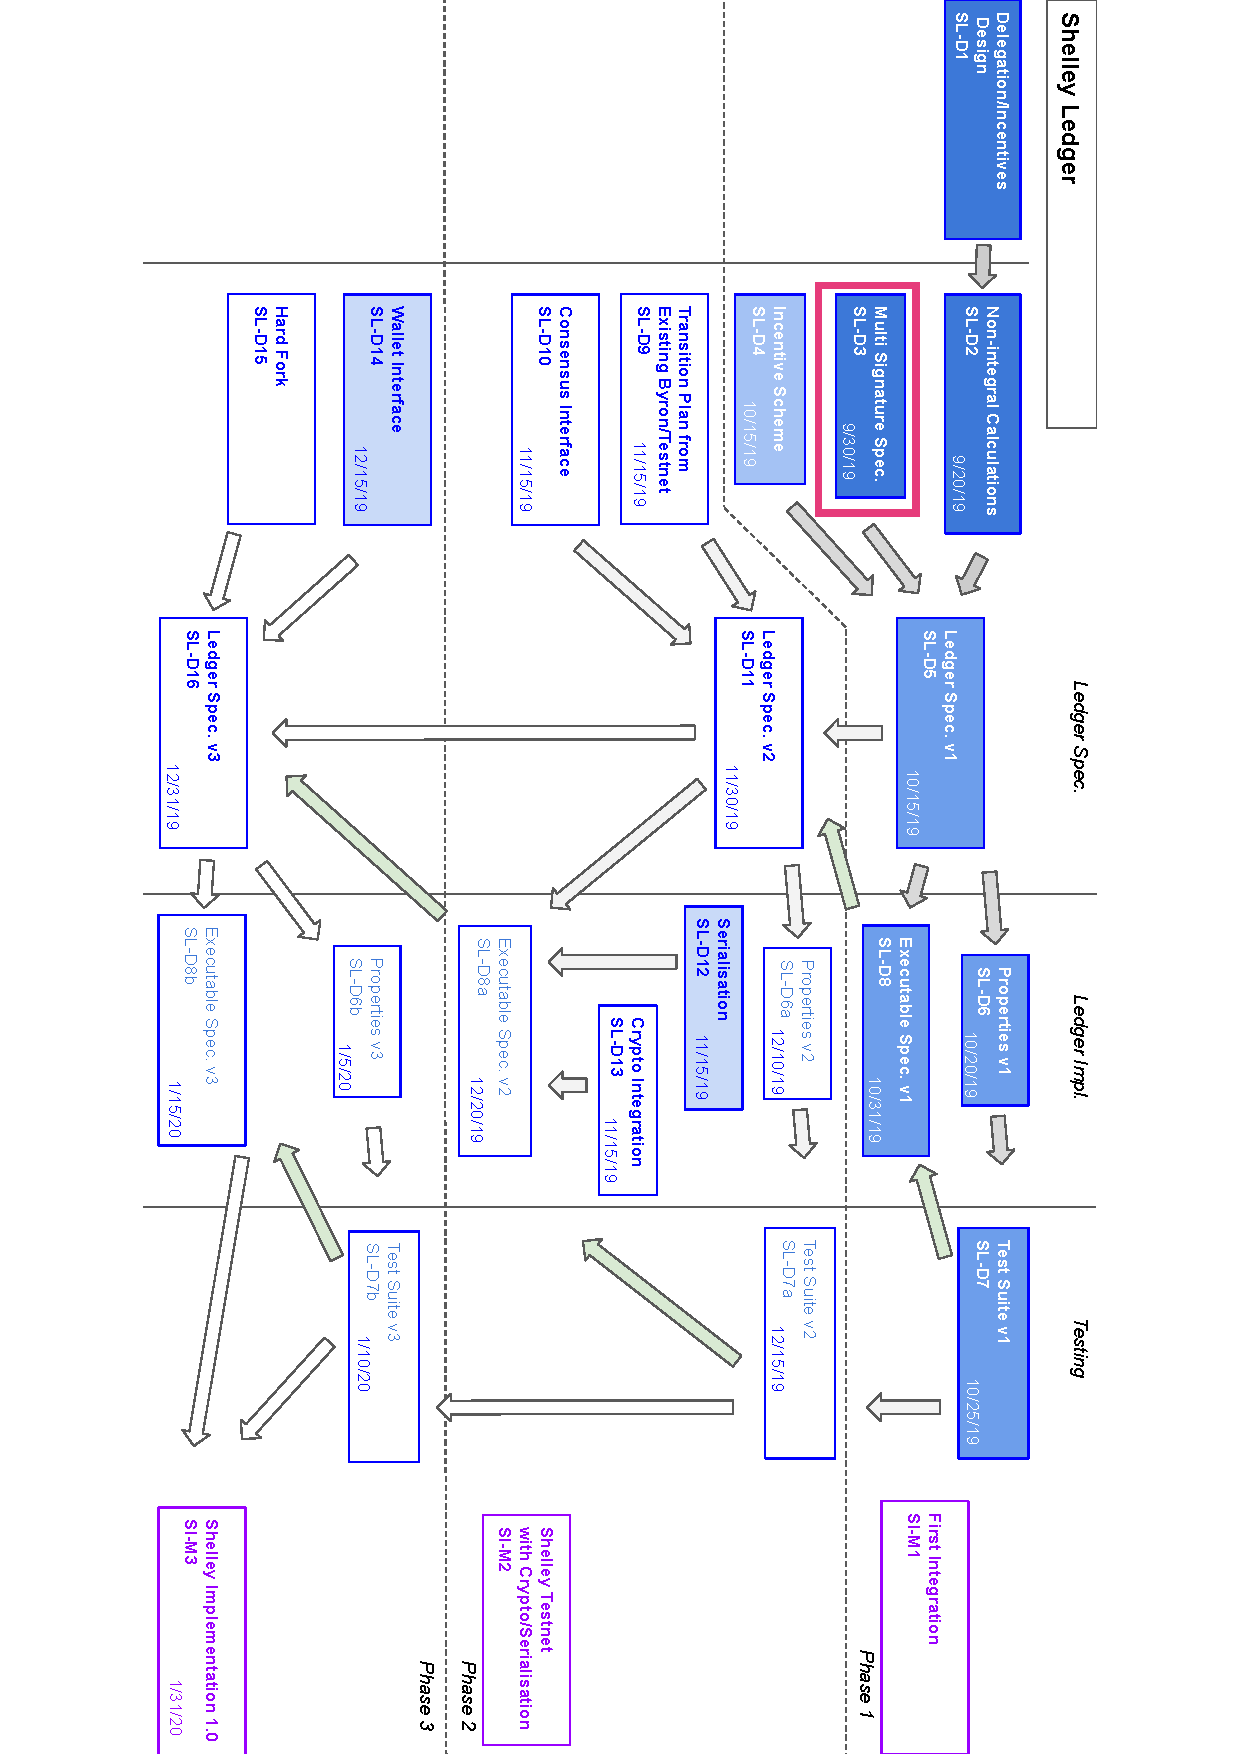
\includegraphics[scale=0.8,angle=90]{d3-depends.pdf}
\caption{Positioning of this Deliverable (outlined in red).}
\end{figure*}
\end{landscape}
\floatstyle{boxed}
\restylefloat{figure}
\cleardoublepage
% \begin{center}
% \large{Executive Summary}
% \end{center}

% \cleardoublepage
\renewcommand{\thepage}{\arabic{page}}
\setcounter{page}{1}

\title{A Formal Specification of a Multi-Signature Scheme using Scripts}

\author{Jared Corduan  \\ {\small \texttt{jared.corduan@iohk.io}} \\
   \and Matthias G\"udemann  \\ {\small \texttt{matthias.gudemann@iohk.io}}}

%\date{}

\maketitle

\begin{abstract}
  This document specifies how to support ``multi-signature'' transactions, that is ones where two or more parties are required
  to authorise the transaction. It  The approach is based on a simple script model, which allows multiple requirements to
  be expressed for a single transaction. It uses only single-step script execution
  and does not require data scripts. We illustrate this by providing two different ways to implement
  such a scheme on top of the Shelley formal ledger specification: \begin{inparaenum}
    \item based on
      Plutus scripts;
    \item
      based on a simple script DSL, for which a native script interpreter can be used.
      \end{inparaenum}
%
  A multi-signature scheme allows an unspent transaction output to be used as an
  input to a new transaction if a pre-defined combination of signatures is
  provided, e.g., if two parties have to sign simultaneously, or two out of three possible
  keys have to be provided, etc.
%
  For an output that is requires a ``multi-signature'', the set of all the keys
  that have signed the transaction is passed to a validation script. In this
  way, the script can decide in a single step whether or not it has a
  combination of keys that will permit the output to be spent correctly.  It is
  possible to supply more signatures than are required to authorise the
  transaction.  In this case, any subset of valid signatures can be used.
\end{abstract}

\tableofcontents
\listoffigures

% \section*{List of Contributors}
% \label{acknowledgements}


\section{Introduction}
\label{sec:introduction}

Under some circumstances, multiple signatures may be required to authorise a transaction, for example, where an account
is held in joint names or is a business account that is held by several business partners.
Depending on the account, it may be that authorisation is required by all signatories or by a single signatory.
This specification for a simple multi-signature scheme
on the formal specification for the Shelley Cardano Ledger~\cite{shelley_spec}.
% which formally specifies the Shelley Cardano ledger.
The main changes from that document are:

\begin{enumerate}
\item Add a new address type for outputs, stake and rewards that require scripts;
\item Add a new witness type to the transaction;
\item Adapt the signature validation in such a way that funds that require a
  multi-signature script can be spent and delegation certificates that require
  multi-signature scripts can be used;
\item Adapt the validation functions to the extended types of
  addresses, transaction inputs and to delegation certificates with scripts.
\end{enumerate}

In this approach for multi-signature, the scripts will receive as input the set of
all the keys that were used to sign the transaction. The script can then check this set
against its own representation of valid combinations of keys that are permitted to unlock the
unspent output.
%
This design means that the scripts are completely stateless and therefore that no data needs to be
supplied to the script apart from the information about which combinations of keys
can legitimately sign the transaction. The design allows for any $n$ of $m$
signatures to be required for each unspent transaction output, where $m, n \ge 0$.

\section{Types}
\label{sec:types}

\begin{figure*}[hbt]
  \emph{Abstract types}

  \begin{equation*}
    \begin{array}{r@{~\in~}l@{\qquad=\qquad}lr}
      script & \Script & \ScriptPlutus\uniondistinct\ScriptMSig\uniondistinct\,\,\cdots  & \text{Representation of a script}
    \end{array}
  \end{equation*}

  \emph{Derived types}

  \begin{equation*}
    \begin{array}{r@{~\in~}l@{\qquad=\qquad}lr}
      \var{addr_{s}} & \AddrScr & \AddrScrBase \uniondistinct \AddrScrEnterprise
                              \uniondistinct \AddrScrPtr & \text{Script address} \\
      \var{addr_{vk}} & \AddrVKey & \begin{array}{l@{~\uniondistinct}l}
                             \AddrVKeyB & \AddrVKeyP \uniondistinct \AddrVKeyE \\
                                    & \AddrVKeyBS
                           \end{array}
                                & \text{Key address}\\
      \var{addr} & \Addr & \AddrScr \uniondistinct \AddrVKey \\
      \var{addr_{rwd}} & \AddrRWD & (\AddrRWDVKey \uniondistinct \AddrRWDScr)
                                                         & \text{Reward address}
    \end{array}
  \end{equation*}

  \emph{Accessor Functions}

  \begin{equation*}
    \begin{array}{r@{~\in~}lr}
      \fun{paymentHK} & \AddrVKey \to \KeyHash_{pay}
      & \text{hash of payment key from addr}\\
      \fun{validatorHash} & \AddrScr \to \HashScr & \text{hash of validator
                                                    script} \\
      \fun{stakeCred_{b}} & (\AddrVKeyB \uniondistinct \AddrScrBase) \to
                          \StakeObject & \text{stake credential from base
                                      addr}\\
      \fun{stakeCred_{r}} & \AddrRWD \to \StakeObject & \text{stake credential
                                                   from reward addr}\\
      \fun{addrPtr} & (\AddrVKeyP \uniondistinct \AddrScrPtr) \to \Ptr &
                                                                         \text{pointer
                                                                         from
                                                                         pointer addr}
    \end{array}
  \end{equation*}

  \emph{Abstract Functions}

  \begin{equation*}
    \begin{array}{r@{~\in~}lr}
      \fun{hashScript} & \Script \to \HashScr & \text{hash a serialized script}
    \end{array}
  \end{equation*}

  \caption{Types for Scripts and Script Addresses}
  \label{fig:types-scripts}
\end{figure*}

In Figure~\ref{fig:types-scripts} the $\Addr$ type of the Cardano Ledger formal
specification~\cite{shelley_spec} is changed to include both public key and
script addresses, split into the sub-types $\AddrVKey$ and $\AddrScr$. Key
addresses, of type $\AddrVKey$, are used as in the original specification;
script addresses contain the hash of the validator script, and are used to
lookup the script. The $\Script$ type is partitioned into subtypes: here,
$\ScriptPlutus$ for Plutus scripts, $\ScriptMSig$ for native interpreter scripts
(see Sections~\ref{sec:plutus-scripts} and~\ref{sec:native-script-interp} for
details).

A transaction output that requires a script carries the hash of the
corresponding validator script. The output can only be spent if the matching
script is provided and validates its input. The necessary information is carried
by the $\AddrScr$ sub-type of $\Addr$ (Figure~\ref{fig:types-scripts}).  This
can therefore be part of a transaction output that consists of a pair of
$\Addr\times\Coin$. Analogously to $\AddrVKey$, $\AddrScr$ also has an
\emph{enterprise} script address sub-type which does not allow staking, as well
as \emph{base} and \emph{pointer} script address sub-types. We will refer to the
parts of an address that is used for payment as the \emph{payment object} and
the part that is used for staking as the \emph{staking reference}. Analogously
to the payment object, the staking reference for an $\AddrScr$ is also a script.
This means that staking can also require a combination of signatures and these
may be different from the combination of signatures that is required for
payment.

The $\fun{hashScript}$ function calculates the hash of the serialized
script. The accessor function $\fun{validatorHash}$ returns the hash of a script
address. The domain of the accessor function $\fun{paymentHK}$ is changed to
public key addresses. The domains of the accessor functions $\fun{stakeHK_b}$,
$\fun{stakeHK_{r}}$ and $\fun{addrPtr}$ are extended to also include the
respective script address variants. The return types are changed to be a staking
reference.

\begin{figure*}[hbt]
  \emph{Transaction Type}

  \begin{equation*}
    \begin{array}{r@{~\in~}l@{\qquad=\qquad}l}
      \var{wit} & \TxWitness & (\VKey \mapsto \Sig, \HashScr \mapsto \Script)
      \\
      \var{tx}
      & \Tx
      & \TxBody \times \TxWitness
      \\
    \end{array}
  \end{equation*}

  \emph{Accessor Functions}

  \begin{equation*}
    \begin{array}{r@{~\in~}lr}
      \fun{txwitsVKey} & \Tx \to (\VKey \mapsto \Sig) & \text{VKey witnesses} \\
      \fun{txwitsScript} & \Tx \to (\HashScr \mapsto \Script) & \text{script witnesses}
    \end{array}
  \end{equation*}

  \emph{Abstract Functions}

  \begin{equation*}
    \begin{array}{r@{~\in~}lr}
      \fun{validateScript} & \Script \to (\Tx \to \Bool) & \text{script interpreter}
    \end{array}
  \end{equation*}
  \caption{Types for Transaction Inputs with Scripts}
  \label{fig:types_defs_multi}
\end{figure*}

Figure~\ref{fig:types_defs_multi} extends the type of a transaction as defined
in the formal ledger specification~\cite{shelley_spec} to carry an additional
witness type. This is achieved by explicitly defining $\TxWitness$ to be a pair
of a public key witness and a script
witness. %\khcomment{I don't understand the difference between a tuple and a $\times$ type.}
The accessor function $\fun{txwits}$ is renamed to $\fun{txwitsVKey}$. The new
accessor function $\fun{txwitsScript}$ returns a map of script hashes to
scripts.  In order for a transaction to be accepted, all the corresponding
scripts need to validate the transaction.

\begin{figure*}[htb]
  \emph{Classification Functions}
  %
  \begin{align*}
    \fun{txinsVKey} & \in \powerset \TxIn \to \UTxO \to \powerset\TxIn & \text{VKey Tx inputs}\\
    \fun{txinsVKey} & ~\var{txins}~\var{utxo} =
    \var{txins} \cap \dom (\var{utxo} \restrictrange (\AddrVKey \times Coin))
    \\
    \\
    \fun{txinsScript} & \in \powerset \TxIn \to \UTxO \to \powerset\TxIn & \text{Script Tx inputs}\\
    \fun{txinsScript} & ~\var{txins}~\var{utxo} =
                        \var{txins} \cap \dom (\var{utxo} \restrictrange (\AddrScr \times Coin))
  \end{align*}
  %
  \caption{Key/Script Classification Functions}
  \label{fig:defs:functions-txins}
\end{figure*}

Figure~\ref{fig:defs:functions-txins} shows the $\fun{txinsVKey}$ and
$\fun{txinsScript}$ scripts, which partition the set of transaction inputs of
the transaction into those that require a private key and those that require a
multi-signature script, respectively.

\section{Ledger Transitions for Multi-Signature}
\label{sec:ledg-trans-multi}

While spending transaction outputs and altering delegation decisions can both
require multi-signature scripts, script validation can be treated in the same
way for both cases. The validation of all witnesses occurs through the UTXOW STS
rule, using the \fun{witsVKeyNeeded} function to collect all the necessary key
signatures and the \fun{scriptsNeeded} function to collect all necessary
multi-signature scripts.

\subsection{Delegation Specific Changes}
\label{sec:deleg-trans-rules}

Staking using multiple signatures requires a change to the type of staking reference from
just a hashed key to either a hashed key or a hashed script. This is
reflected in the type of $\StakeCreds$ (which replaces the previous
$\type{StakeKeys}$ type) and the new $\StakeObject$ type, % (which describes either a key or a script used for staking),
as shown in
Figure~\ref{fig:delegation-state-type}.

\begin{figure}
  \emph{Delegation Types}
    \begin{equation*}
      \begin{array}{r@{~\in~}l@{\qquad=\qquad}lr}
        \var{stakeCred} & \StakeObject & (\KeyHash_{stake} \uniondistinct
                                            \HashScr) \\
        \var{regCreds} & \StakeCreds & \StakeObject \mapsto \Slot \\
      \end{array}
    \end{equation*}
    %
  \emph{Delegation States}
  %
  \begin{equation*}
    \begin{array}{l}
    \DState =
    \left(\begin{array}{r@{~\in~}lr}
      \var{stkCreds} & \StakeCreds & \text{registered stake delegators}\\
      \var{rewards} & \AddrRWD \mapsto \Coin & \text{rewards}\\
      \var{delegations} & \StakeObject \mapsto \KeyHash_{pool} & \text{delegations}\\
      \var{ptrs} & \Ptr \mapsto \StakeObject & \text{pointer to staking reference}\\
      \var{fGenDelegs} & (\Slot\times\VKeyGen) \mapsto \VKey & \text{future genesis key delegations}\\
      \var{genDelegs} & \VKeyGen \mapsto \VKey & \text{genesis key delegations}\\
          \end{array}\right)
    \end{array}
  \end{equation*}
  %
  \emph{Certificate Accessor functions}
  %
  \begin{equation*}
  \begin{array}{r@{~\in~}lr}
    \cwitness{} & \DCert \to \StakeCreds & \text{certificate witness}
  \end{array}
  \end{equation*}
  \caption{Delegation State type}
  \label{fig:delegation-state-type}
\end{figure}

\textbf{Note:} In contrast to staking reference delegation, staking pools
themselves cannot use multi-signature schemes. Otherwise, the lightweight
certificates that are used for delegation from the pool to the KES hot keys would also need to be
script witnesses. This is undesirable since these certificates need to be included in each header,
but headers are required to have a minimal and fixed size. %\khcomment{What size
                                                           %is acceptable?}

\subsection{UTXOW Transition Rule}
\label{sec:utxow-transition}

The UTXOW extended transition system of~\cite{shelley_spec} is shown in
Figure~\ref{fig:rules:utxow-multi-sig}. The constraint on the set of required
witnesses is relaxed in such a way that \emph{redundant} signatures can be
supplied in the transaction. %\khcomment{redundant meaning ``not required'' or
                             %``duplicate''?}
The set of verification keys is passed to the validator script
via the concrete implementation of $\fun{validateScript}$ for the specific
script type.
%
The set of all validator scripts of $\fun{txwitsScript}~(\fun{txins}~tx)$ is
checked for:

\begin{enumerate}
\item equality of the hashed script with the hash that is stored in the output to spent;
\item that the script validates the transaction; and
\item that it is precisely the set of the scripts required for the transaction
  (as returned from $\fun{scriptsNeeded}$).
\end{enumerate}

\begin{figure}[htb]
  \begin{equation}
    \inference[UTxO-wit]
    {
      (utxo, \wcard, \wcard) \leteq \var{utxoSt} \\~\\
            \forall \var{hs} \mapsto \var{validator} \in \fun{txwitsScript}~{tx},\\
      \fun{hashScript}~\var{validator} = \var{hs} \wedge
      \fun{validateScript}~\var{validator}~\var{tx}\\~\\
      \fun{scriptsNeeded}~\var{utxo}~\var{tx} = \dom (\fun{txwitsScript}~{tx})
      \\~\\
      \forall \var{vk} \mapsto \sigma \in \txwitsVKey{tx},
      \mathcal{V}_{\var{vk}}{\serialised{\txbody{tx}}}_{\sigma} \\
      \fun{witsVKeyNeeded}~{utxo}~{tx} \subseteq \{ \hashKey \var{vk} \mid
      \var{vk}\in\dom{(\txwitsVKey{tx})} \}\\~\\
      {
        \begin{array}{l}
        \var{utxoEnv}
        \end{array}
      }
      \vdash \var{utxoSt} \trans{\hyperref[fig:rules:utxo-shelley]{utxo}}{tx} \var{utxoSt'}\\
    }
    {
      \begin{array}{l}
        \var{utxoEnv}
      \end{array}
      \vdash \var{utxoSt} \trans{utxow}{tx} \varUpdate{\var{utxoSt'}}
    }
  \end{equation}
  \caption{UTxO with Witnesses and Multi-Signatures}
  \label{fig:rules:utxow-multi-sig}
\end{figure}

Multi-signature staking also causes reward accounts to be locked by a multi-signature
scheme. This means that in order to allow for spending of rewards accumulated in
a multi-signature rewards account, we also need to validate the required
script. This is done in a predicate in the UTXOW rule which checks that for each
withdrawal of a transaction which uses a multi-script rewards account, there
exists a corresponding script that matches the hash in the reward address and that also
validates the transaction. Because of the changes to the staking reference type,
the original function $\fun{witsNeeded}$ is changed as shown in
Figure~\ref{fig:functions-witnesses}. Figure~\ref{fig:functions-witnesses} also shows the function
$\fun{scriptNeeded}$ that computes the required script hashes from the set of
spent inputs that are locked by scripts and the consumed withdrawals that are locked by scripts.

\begin{figure}[htb]
  \begin{align*}
    & \hspace{-0.8cm}\fun{witsVKeyNeeded} \in \UTxO \to \Tx \to (\VKeyGen\mapsto\VKey) \to
      \powerset{\KeyHash}
    & \text{required keyhashes} \\
    &  \hspace{-0.8cm}\fun{witsVKeyNeeded}~\var{utxo}~\var{tx}~\var{dms} = \\
    & ~~\{ \fun{paymentHK}~a \mid i \mapsto (a, \wcard) \in \var{utxo},~i\in\fun{txinsVKey}~{tx} \} \\
    \cup & ~~
           \left(\{\fun{stakeCred_r}~a\mid a\mapsto \wcard \in \AddrRWDVKey
      \restrictdom \txwdrls{tx}\} \cap \KeyHash_{Stake}  \right)\\
    \cup & ~~\{\cwitness{c} \mid c \in \txcerts{tx}\}~\cup \\
    \cup & ~~\fun{propWits}~(\fun{txup}~\var{tx}) \\
    \cup & ~~\bigcup_{\substack{c \in \txcerts{tx} \\ ~c \in\DCertRegPool}} \fun{poolOwners}~{c}
  \end{align*}
  \begin{align*}
    & \hspace{-0.5cm}\fun{scriptsNeeded} \in \UTxO \to \Tx \to
      \powerset{\HashScr}
    & \text{required script hashes} \\
    &  \hspace{-0.5cm}\fun{scriptsNeeded}~\var{utxo}~\var{tx} = \\
    & ~~\{ \fun{validatorHash}~a \mid i \mapsto (a, \wcard) \in \var{utxo},\\
    & ~~~~~i\in\fun{txinsScript}~{(\fun{txins~\var{tx}})}~{utxo}\} \\
    \cup & ~~\left(\{ \fun{stakeCred_{r}}~\var{a} \mid a \in \dom (\AddrRWDScr
           \restrictdom \fun{txwdrls}~\var{tx}) \} \cap \HashScr\right) \\
    \cup & ~~\{\AddrScr \cap \fun{cwitness}~\var{c} \mid c \in \fun{txcerts}~\var{tx}\}
  \end{align*}
  \caption{Required Witnesses}
  \label{fig:functions-witnesses}
\end{figure}

\section{Implementation of Script-Based Multi-Signature}
\label{sec:altern-impl}

There are different implementation possibilities for the introduced
multi-signature scheme. Section~\ref{sec:plutus-scripts} describes an
implementation based on Plutus~\cite{plutus_eutxo} which uses only simple
scripts, without redeemer or data
scripts. Section~\ref{sec:native-script-interp} describes an alternative
implementation that supports validation using a
native implementation for a script-like DSL.

\subsection{Plutus Scripts}
\label{sec:plutus-scripts}

\begin{figure*}[hbt]
  \emph{Abstract Type}

  \begin{equation*}
    \begin{array}{r@{~\in~}lr}
      pendingTx & \PendingTx & \text{information about pending Tx}
    \end{array}
  \end{equation*}

  \emph{Abstract Functions}

  \begin{equation*}
    \begin{array}{r@{~\in~}lr}
      \fun{validateScript} & \ScriptPlutus \to (\Tx \to \Bool) & \text{Plutus script
                                                               interpreter} \\
      \fun{validate} & () \to () \to (\PendingTx \to \Bool) & \text{Plutus
                                                            validator script type}
    \end{array}
  \end{equation*}
  \caption{Implementation based on Plutus Scripts}
  \label{fig:types_defs_plutus}
\end{figure*}

$\PendingTx$ is a representation of the pending transaction. In particular, this
information contains the set of keys that signed the transaction. The function
$\fun{txPending}$ constructs the necessary information about a transaction
which can be passed as value of type $\PendingTx$ to the validator script.

In order to spend funds locked by a multi-signature script, the validator
scripts need to validate the transaction. The abstract function $\fun{validate}$
corresponds to such a Plutus validator script. Its type consists of two
parameters of unit type and one parameter of type $\PendingTx$; its return type
is Boolean. The first two input parameters correspond to the redeemer and the
data scripts which are used in the full extended UTxO model for
Plutus~\cite{plutus_eutxo}. As those values are not required for simple
multi-signature, we use the unit type for them. The Boolean return type signals
whether the script succeeded in validating the transaction. The function
$\fun{validateScript}$ specialized for $\ScriptPlutus$ takes a Plutus script
representation and a $\PendingTx$ value, and evaluates the script using the
Plutus interpreter.

The following is a possible Plutus implementation of a simple $m$ out of $n$
multi-signature validation script. The type $\type{MultiSig}$ is a list of keys
and a threshold value.

\begin{verbatim}
import qualified Language.PlutusTx            as P
import           Ledger.Validation            as V

data MultiSig = MultiSig
                { signatories :: [Ledger.PubKey]
                -- ^ List of public keys of people who may sign the transaction
                , requiredSignatures :: Integer
                -- ^ Minimum number of signatures required to unlock
                --   the output (should not exceed @length signatories@)
                --   n.b., should also check that this is >= 0
                }

validate :: MultiSig -> () -> () -> PendingTx -> Bool
validate multiSig@(MultiSig keys num) () () p =
    let present = P.length (P.filter (V.txSignedBy p) keys)
    in present `P.geq` num
\end{verbatim}

The above Plutus script takes a parameter \var{multiSig} of type
$\type{MultiSig}$.  This is a list of keys $\var{keys}$ and a threshold $num$
that indicates how many of the keys are required as signatures. When the
validation script is called, it computes the length of the list of keys in $keys$ which correctly signed
the transaction. If this number is greater than or equal to \emph{num},
then sufficient signatures are present. It follows that, since
\var{hkeys} is a value of type \type{MultiSig}, partial application of
$\fun{validate}~multisig$ will return a correctly typed validator script
as defined by Figure~\ref{fig:types_defs_plutus}.

\subsection{Native Script Interpreter}
\label{sec:native-script-interp}

\begin{figure*}[hbt]
  \emph{MultiSig Type}

  \begin{equation*}
    \begin{array}{rll}
      \var{msig} & \in & \type{RequireSig}~\KeyHash\\
      & \uniondistinct &
         \type{RequireAllOf}~[\ScriptMSig] \\
      & \uniondistinct&
         \type{RequireAnyOf}~[\ScriptMSig] \\
      & \uniondistinct&
        \type{RequireMOf}~\N~[\ScriptMSig]
    \end{array}
  \end{equation*}

  \emph{Functions}

  \begin{align*}
    \fun{validateScript} & \in\ScriptMSig\to\Tx\to\Bool & \text{validate native
                                                          script} \\
    \fun{validateScript} & ~\var{msig}~\var{tx}= \\
                         & \textrm{let}~\var{vhks}\leteq \{\fun{hashKey}~vk \vert
                           vk \in \fun{txwitsVKey}~\var{tx}\} \\
                         & \fun{evalMultiSigScript}~msig~vhks\\
  \end{align*}
  \begin{align*}
    \fun{evalMultiSigScript} & \in\ScriptMSig\to\powerset\KeyHash\to\Bool & \\
    \fun{evalMultiSigScript} & ~(\type{RequireSig}~hk)~\var{vhks} =  hk \in vhks \\
    \fun{evalMultiSigScript} & ~(\type{RequireAllOf}~ts)~\var{vhks} =
                              \forall t \in ts: \fun{evalMultiSigScript}~t~vhks\\
    \fun{evalMultiSigScript} & ~(\type{RequireAnyOf}~ts)~\var{vhks} =
                              \exists t \in ts: \fun{evalMultiSigScript}~t~vhks\\
    \fun{evalMultiSigScript} & ~(\type{RequireMOf}~m~ts)~\var{vhks} = \\
                             & m \leq \Sigma
                               (\textrm{card} \{ t s.t. t \leftarrow ts \wedge \fun{evalMultiSigScript}~\var{t}~\var{vhks}
%                               \left(
%                               [\textrm{if}~(\fun{evalMultiSigScript}~\var{t}~\var{vhks})~
%                               \textrm{then}~1~\textrm{else}~0\vert t \leftarrow ts]
%                               \right)
  \end{align*}

  \caption{Implementation based on Native Scripts}
  \label{fig:types-msig}
\end{figure*}

An alternative implementation for multi-signature scripts is an embedding of the
script as a data type that can then be interpreted
directly. Figure~\ref{fig:types-msig} shows the types and functions
that are needed for such a native script implementation. The type $\ScriptMSig$ is defined as a
tree-structure which is either a single signature leaf node or a list of values
of type $\ScriptMSig$.  This either requires all signatures to be validated, at
least one of the signatures to be validated, or at least the threshold value of $m$
signatures to be validated.

\subsection{Lower Level Implementation Details}
\label{sec:lower-level-impl}

For each new type of witness, there will be a requirement to represent such a
witness on-chain and allow for identification when deserializing such a
witness. For this, there will be a language-specific tag for each witness (and
staking reference) in its serialized form. This tag will also be part of the
hash to allow for easy identification of the language type.

As an example, one could tag key hash payment object and staking references with
the tag $0$, native multi-signature scripts with the tag $1$, and simple Plutus scripts with the tag
$2$. Every new language would require a new tag. Changes to the payment or staking reference details
that are treated \emph{within} an existing language
framework would be changed via a software update, rather than an additional tag.

\section{Summary}
\label{sec:summary}

The script-based multi-signature scheme that is presented here does not require the scripts
to use any cryptographic primitives. Rather, it requires only the ability to compare the
required keys to those that actually signed the transaction. The worst-case
potential calculation cost can therefore be calculated statically in advance and
can be added to the transaction fees or as gas cost. %\khcomment{Assumes
                                                     %transactions are
                                                     %independent.}
The scripts can be realized
with only limited functionality  requirements for the script language.
%
The necessary extensions to the data types in the Shelley
specification~\cite{shelley_spec} are relatively simple. They consist
mainly of introducing additional optional data types for payment objects or
staking references.

The relaxation on accepting a superset of the strictly required signatures
potentially allows the creation of transactions with an arbitrary number of signatures. This
could then be a possible attack vector. The number of signatures should be taken
into account in some way in the calculation of the transaction fee.

There are two proposed implementation schemes, one based on Plutus, the other on
a script-like integration as DSL for a native interpreter. Both follow the same
strategy for integration: extending addresses, defining witnesses and
specializing the script validation function. If the Plutus approach is not
viable for any reason, e.g., script size or readiness of library, only the
native script implementation could be pursued instead.

\addcontentsline{toc}{section}{References}
\bibliographystyle{habbrv}
\bibliography{references}

\end{document}


%%% Local Variables:
%%% mode: latex
%%% TeX-master: t
%%% End:
